\documentclass[tikz]{standalone}
\usepackage{tikz}
\usetikzlibrary{patterns}


\begin{document}
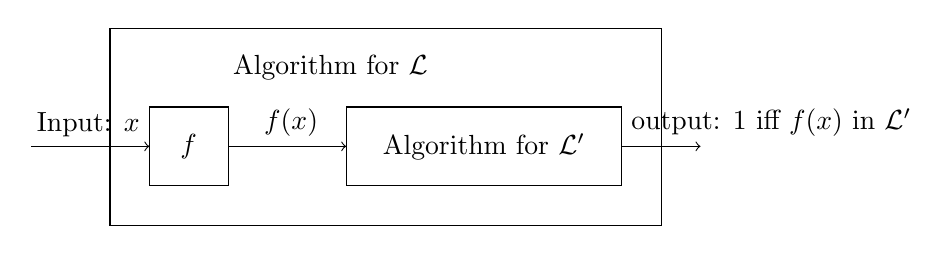
\begin{tikzpicture}

	\draw (0,0) rectangle (7,2.5);
	\node at (2.8,2.0) {Algorithm for $\mathcal{L}$};
	\draw (0.5,0.5) rectangle (1.5,1.5) node at (1,1) {$f$};        \draw (3,0.5) rectangle (6.5,1.5);
	\node at (4.75,1) {Algorithm for $\mathcal{L}'$};
	\draw[->] (-1,1) -- (0.5,1) node[above left] {Input: $x$};
	\draw[->] (1.5,1) -- (3,1);
	\node at (2.3, 1.3) {$f(x)$};
	\draw[->] (6.5,1) -- (7.5,1);
	\node at (8.4,1.3) {output: $1$ iff $f(x)$ in $\mathcal{L}'$};

\end{tikzpicture}
\end{document}